\documentclass[12pt,a4paper]{ltxdoc}
\usepackage{lmodern}			% Usa a fonte Latin Modern			
\usepackage[T1]{fontenc}		% seleção de códigos de fonte.
\usepackage[utf8]{inputenc}		% determina a codificação utilizada (conversão automática dos acentos)
\usepackage{hyperref}  			% controla a formação do índice
\usepackage{parskip}			% espaçamento entre os parágrafos
\usepackage{microtype} 			% para melhorias de justificação
\usepackage{morefloats}			% permite mais floats
\usepackage{setspace}
%\singlespacing
\onehalfspacing
%\doublespacing
%\setstretch{1.1}

%\documentclass[10pt,a4paper]{article}
%\usepackage[utf8]{inputenc}
\usepackage[english]{babel}
\usepackage{amsmath}
\usepackage{amsfonts}
\usepackage{amssymb}
\usepackage{graphicx}
%Alessandro input: makecell package to permite line break inside tables
\usepackage{makecell}
\usepackage[alf]{abntex2cite}	% citacoes
\graphicspath{ {./images/} }

\title{Automated Verification Applied to Stand-alone Solar Photovoltaic Systems: Optimal Sizing and Project Validation}
\author{Alessandro Bezerra Trindade \thanks{Federal University of Amazonas, Av. Rodrigo Octavio 3000, Coroado, Faculdade de Tecnologia, Campus Universitário, Manaus-AM, Brazil, alessandrotrindade@ufam.edu.br}}
\date{}

\begin{document}

\maketitle

\begin{abstract}
xxxx

Keywords: Automated verification, model checking, energy systems, solar photovoltaic systems, off-grid systems. 
\end{abstract}

\begin{abstract}
xxxx

Palavras-chave:  ab c 
\end{abstract}

\section{Introduction}
Lack of access to clean and affordable energy is considered a core dimension of poverty~\cite{Hussein2012}. Progress has been made worldwide; in particular, the number of people without electricity access fell below 1 billion threshold for the first time in 2017~\cite{IEAweo2018}. In order to provide universal electricity for all, decentralized systems led by solar photovoltaic (PV) in off-grid and mini-grid systems will be the lowest-cost solution for three-quarters of the additional connections needed; and grid extension will be the standard especially in urban areas~\cite{IEAweo2018}.

In order to simulate or evaluate a PV system, there are various specialized tools available in the market, e.g. RETScreen, HOMER, PVWatts, SAM and Hybrid2 \cite{Pradhan,Swarnkar,NRELDobos,NRELBlair,Mills}; and even general purpose simulation tools, e.g. PSpice, Saber or MATLAB/Simulink package \cite{Gow1999,Benatiallah2017}. However, those tools are based on simulation models, which are employed before the system design is concluded; it has the drawback of an incomplete coverage since verification of all possible combinations and potential failures of a system is unfeasible~\cite{ClarkeHV18}.

Formal methods based on \textit{model checking} can offer a great potential to obtain a more effective design process of PV systems~\cite{ClarkeHV18}.

///////////

According to \cite{Coelho} there are presently 1.3 billion people with no access to electricity worldwide. The definition of energy access usually includes both electricity access and access to modern fuels for cooking and heating, in order to replace traditional biomass. Increased access to energy allows economic growth and poverty alleviation \cite{Karekesi}. 

Among the options of renewable sources, there are hydro, wind, and solar photovoltaic (PV). Only a niche market a few years ago, PV are now becoming a mainstream electricity provider, changing the way the world is powered. Based in data from \cite{EPIA}, there was an increase of approximately 30\% from 2013 to 2014 in terms of new installations of PV. The use of the power generation technology with renewable energy source is developing rapidly due to the industrial development \cite{Yatimi}. The renewable energy leads to an advance all over the world by protecting the environment: it is clean (low greenhouse gases emissions), operating silently, long lifetime, low maintenance, absence of fuel cost and inexhaustible \cite{Noroozian}. Renewable energy, and particularly the power generation from solar energy using photovoltaic (PV) panels, has emerged as an alternative to fossil or nuclear fuel generation. The increase in a number of PV systems installed all over the world brings the need for proper modeling and simulation tools for researcher and practitioners involved in their application. 

In order to validate or even simulate a potential PV solution, there are a myriad of tools. However, to the best of our knowledge, this work can be the first work to perform automated verification of a solar PV off-grid project solution.  

According to \cite{SEIA} and \cite{Chauhan}, solar is the most abundant source of renewable energy on earth. In SPV system, solar radiations are captured from the sun and turned into electricity using SPV cells made of silicon and other materials. SPV systems can be classified into grid-connected and stand-alone systems. At this proposal, only off-grid or stand-alone systems will be considered. The utilization of solar energy in off-grid mode has the potential to meet the energy need for remote rural areas of developing countries.  

The PV cell in a solar photovoltaic system, as defined in \cite{Rawat}, is a semiconductor device, which directly converts the solar radiation into electrical energy. Apart from PV modules; the PV systems consist of battery bank, controller, and inverter, plus the load. Moreover, the optimum sizing of these devices is important for reliable operation. Therefore, these systems need to be designed properly according to the site, land area available, load requirement, load pattern, environmental conditions and economics in order to utilize available resources efficiently and economically \cite{Rawat}. 

\subsection{Problem's Definition}
 
In order to address different aspects of a SPV project, there is a myriad of public domain and commercial software available. According to \cite{Brooks}, the capabilities of these tools range from simple solar resource and energy production estimative, to site survey and system design tools, to complex financial analysis software (with optimization). Some tools also provide support to rebate programs applications and tax incentives (specific to each country or region), while other programs and worksheets focus on the technical aspects of system sizing and design.  

Manufacturers and integrators have yet their proprietary software to perform various system sizing, with the drawback of include just their own products among the possibilities of choice, what restrict the solution. 

Changing the subject to the design of complex systems, more time is spent on verification than on construction, as shown in \cite{Baier}. Formal methods based on model checking offer great potential to obtain a more effective and faster verification in the design process. Programs, and more generally computer systems, may be viewed as mathematical objects with behavior that is, in principle, well determined. This makes it possible to specify programs using mathematical logic, which constitutes the intended (correct) behavior. Then, one can try to give a formal proof or otherwise establish that the program meets its specification, as defined by \cite{Trindade}. 

This area of research is referred as formal methods as defined in \cite{Clarkeetal}. Their aim is to establish system correctness with mathematical rigor. 

In the recent decades, research in formal methods has led to the development of very promising verification techniques that facilitate the early detection of bugs in order to ensure the correctness of the system. 

Model-based verification techniques are based on models that describe the possible system behavior in a mathematically precise and unambiguous manner. Thus, such problems as incompleteness, ambiguities, and inconsistencies, which normally are discovered only in later stages of the design, can be detected in advance, as described by \cite{Trindade}. Algorithms can verify the system model through systematically explore all their states. 

\subsection{Objectives}
Bringing this idea to the field of solar photovoltaic systems, instead of finding a bug or a software inconsistence, the present work aim to verify a complete PV system project, informing in which condition the project do not meet user requirements or will fail. Among the non-deterministic variables evaluated, is it worth to mention environmental issues (like solar irradiance, and temperature), and the variation of the electrical load (power consumption) or the battery' state of charge, as shown in Fig.\ref{fig:flowchartgeneral}. That is the main contribution of this paper.

\begin{figure}[h]
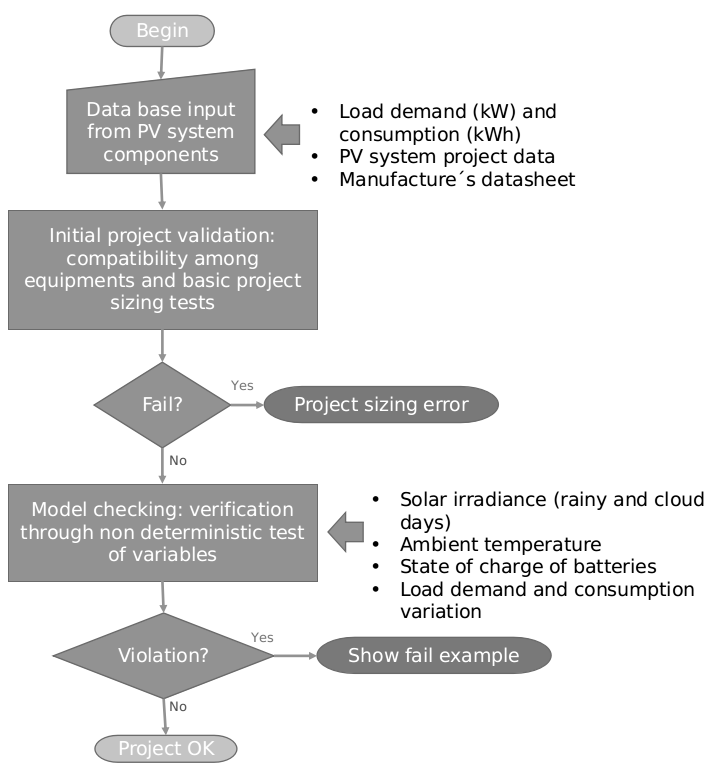
\includegraphics[width=0.8\textwidth]{flowchart_verification.png}
\centering
\caption{Flowchart of the proposed computer verification of PV systems}
\label{fig:flowchartgeneral}
\end{figure}

The framework provided at this paper outlines the requirements, the process and the mathematical modeling to perform automated formal verification of a complete PV off-grid system, using the satisfiability modulo theories (SMT)-based verification method.
 
To the best of our knowledge, this is the first work to use an SMT-based verification tool to solve this kind of problem. 

The implementation of the ideas will be done with the efficient SMT-based bounded model checker (ESBMC) tool that uses the front-end of the C Bounded Model Checker (CBMC) or the clang-based front-end, which permits to describe the problem as a C/C++ language code.

The CBMC, it is notable its prominence through international awards received in competitions. In the works related to the CBMC, much of the research is focused on the improvement of the tool (as software and hardware verifier) and its performance in the competitions, without addressing, however, the question of PV system validation, as can be seen in \cite{Kroening}. For example, in \cite{Schrammel2017}, CBMC received an extension to perform verification of embedded software. 

ESBMC was developed to perform bounded model checks on both sequential and concurrent programs using a range of SMT solvers, and has a proven track of bug finding in real-world applications \cite{Cordeiro}, \cite{Ramalho}. The tool also implements a technique to prove the correctness of (some) unbounded programs, the k-induction algorithm; this approach has been applied to a large number of benchmarks and has produced more correct results than similar competing tools \cite{GadelhaSBMF}, \cite{GadelhaK}. \cite{Trindade} show that is possible to perform the partitioning of hardware-software (optimization) using ESBMC as well. \cite{Bessa} show that is possible to use ESBMC to check the stability of digital control systems with uncertainty. In addition, \cite{Abateetal2017} show the approach to synthesize safe digital feedback controllers for physical plants represented as linear, time invariant models. However, the use of ESBMC to verify PV systems is unprecedented. 

Concerning modeling and simulation of electrical energy systems, \cite{Kremers} used an agent-base model approach to evaluate the effect of loads (refrigerators mainly), shedding, grids, wind power generation, and smart grids, in a dynamic integral multi-scale case study. However, that is a software development approach for the simulation of complex systems, without the formalism of automated verification. 

In the other hand, the use of formal verification related to modeling and validation or even simulation of power systems or power networks is a young theme of research. According \cite{Abateetal2014}, where articles from seminars were issued at this thematic, the actual focus is on optimization and control of microgrids, HVAC systems (diagnostics and maintenance), models of generic wind turbine generation, modeling of transmission networks, and verification of smart grids. In addition, according with \cite{Abate2017}, recent research has attempted to formalize and implement a formal study of large population of PV panels (very common in European Union). The focus have been the modeling of the dynamics of PV panels and their interaction with the power grid. Those models do not use battery array, for example. 

Therefore, the present work unites the versatility and power of the formal models, applied to a formal verification tool, with individual PV systems (off-grid), which is the most indicated and common option to solve the problem of energy in developing countries. Especially those that have isolated communities, either for long distances of the great centers, or for being riverside. This work includes, based on its off-grid characteristic, batteries and charge controllers, differently of on-grid systems of related work. 

\subsection{Contributions}
This paper makes two main contributions. % Firstly, we describe a modular modeling of each component of a PV system by means of mathematical models that can be encoded into fragments of first-order theories supported by software model checkers. Secondly
Firstly, we propose an algorithm written in language C that implements the automated verification method which formally checks the sizing and the operation of a given stand-alone PV system. Secondly, we evaluate the verification method by comparing three state-of-the-art model checkers in five real case studies. %Thirdly, experimental results show that this proposed approach can find subtle design errors in stand-alone PV systems, which are not easily detected by other approach based on simulation.

Our work makes two major contributions. Firstly, the use of automated symbolic verification in electrical systems was uncommon in recent prior studies~\cite{abs-1811-09438}, and specifically their use in synthesizing PV sizing is unprecedented. Here, a list of PV components %(i.e., PV panels, charge controllers, inverters, and batteries) 
can be fed to our proposed synthesis method together with user requirements and environment constraints, and our synthesis algorithm based on symbolic model checking can find the optimal solution in technical and economical terms. Secondly, we evaluate different state-of-art symbolic software verifiers with the goal of obtaining the best performance in our verification back-end for synthesizing optimal PV systems.

\subsection{Related Work}
The conversion of traditional power grid into a smart grid, a fundamental example of a Cyber-Physical System (CPS), raises a number of issues that requires novel methods and applications. In 2012, a Chinese smart grid implementation was considered as case study to address the verification problem for performance and energy consumption~\cite{Yukseletall2012}. The authors employed a stochastic model checking approach and presented a modelling and analysis study using PRISM~\cite{KwiatkowskaNP11}. The focus of this study was on how CPs integrate information and communication technology functions to the physical elements of a system for monitoring and controlling purposes; here the authors employed automated verification of certain quantitative properties of the system, as 	probability	of	node	failure	in	the	long run, impact	of	repair	service	on	the	failure	risk, and expected energy consumption. %, with no interest in power generation or even solar PV systems.

In 2015, an approach for applying Monte-Carlo simulation to power system protection schemes presented limitations of incomplete coverage of all possible operating conditions~\cite{Sengupta2015}. The authors proposed an automated simulation-based verification technique to verify correctness of protection settings efficiently using hybrid automata-temporal-logic framework. The initial focus was on relay operations and test-case generation to ensure early detection of design errors. %The study was limited to power system protection and did not deal with electricity generation or even solar PV systems.

Other related studies from 2015 include a framework named Modana to achieve an integrated process from modeling with SysML/MARTE to analysis with statistical model checking for CPSs in terms of non-functional properties such as time and energy~\cite{Cheng2015}. In order to demonstrate Modana's capability, the authors modelled energy-aware buildings as a case study, and discussed the analysis on energy consumption in different scenarios. The focus here is on smart buildings and HVAC (heating, ventilation, and air conditioning) systems. %The research did no deal with solar PV systems. 
 
In 2017, a researcher suggested the application of formal methods to verify and control the behavior of computational devices interacting over a shared and smart infrastructure~\cite{Abate2017}. The author discussed the aggregation of large populations of thermostatically-controlled loads and of PV panels, and the corresponding problems of energy management in smart buildings, of demand-response on smart grids, and respectively of frequency stabilization and grid robustness. The focus was on controlling the behavior of components, thereby verifying the smart grid as a ``system of systems'' within the context of ``internet of things''. The author used approximate model checking of stochastic and hybrid models.

In 2018, a verification methodology was proposed for the Cyber Physical Energy Systems (CPES) with applications to PV panels and its distributed power point tracking~\cite{Driouich2018}. This approach relied on representing unpredictable behavior of the environment to cover all possible feasible scenarios. The simulation results obtained by JModelica covered the system's complete dynamic behavior; however, it was evident the time consuming issue with almost three days of computer effort to verify the design space of one operation hour of the PV panels behavior. %The work did not include the other components of a stand-alone solar PV system.

Another work from 2018 was the approach to modeling smart grid components using a formal specification. The authors used a state-based formal specification language named Z; they demonstrated the application of Z to four smart grid components~\cite{Akram2018}. The presented formal specification can be considered as a first step towards modeling of smart grid using formal methods. The starting point of this study was that a smart home can be considered as an integrated system consisting of various objects and system, which communicates and interacts with each other. This approach is base on Petri nets and from the premise that modeling of the smart home leads to clear understanding of the overall behavior of the smart grid.

\subsection{Thesis Organization}
The remainder of this paper is organized as follows: Sect. 2 gives a background of solar PV systems. Section 3 describes the design and validation of a solar PV system. Section 4 describes the formal mathematical modeling of a generic PV system. Section 5 presents the automated verification theory, including details of the ESBMC process. The methodology is presented at Section 6. Section 7 discusses the related work. Section 8 presents the conclusion and describes future work. At the end of the paper, there is a list of all nomenclatures used at the text. 

\section{Background}
\subsection{Solar Photovoltaic System }
According to \cite{Roy}, a PV system is designed to give the electric supply to a load. This load can be either Alternate Current (AC) type or Direct Current (DC) type. Electric supply can be needed either in daytime or evening time (in particular cases, in both times). The most basic PV system can give supply only in daytime.  For night hours or rainy days, one needed to have batteries, where power can be stored and used \cite{Gules}. 

PV systems are broadly classified into three distinct types, as described by \cite{Mohanty}: 

\begin{itemize}
\item Standalone systems, where the energy is generated and consumed in the same place and which does not interact with the main grid. Normally, the electricity consuming/utilizing device is part of the system, i.e., solar home systems, solar street lighting system, solar lanterns, and solar power plants; 
\item Grid-connected systems, where the solar PV system is connected to the grid. The grid-connected system can be either a grid-tied system, which can only feed power into the grid and such system cannot deliver power locally during blackouts and emergencies since these systems have to be completely disconnected from the grid and have to be shut down as per national and international electrical safety standards. Some grid-connected PV systems, with energy storage, can also provide power locally in an islanding mode; 
\item Solar PV hybrid system: In a hybrid system, another source(s) of energy, such as wind, biomass or diesel, can work together with the solar PV system to provide the required demand. In such type of system, main objective is to bring more reliability into the overall system at an affordable way by adding one or more energy sources.
\end{itemize}
 
Specifically concerning isolated communities, depending on the type of load, cost, resources availability, and requirements of the load, standalone systems can be split into several categories, which are described in this section. As the goal of this Thesis is just the solutions aimed to isolated/ off-grid application, therefore it is not considered the on-grid or hybrid configurations.
 
There is a resource, called maximum power point tracking (MPPT), which is an electronic control mechanism that maintains the PV operating in a voltage that correspond to the voltage of maximum power, which maximizes the transfer of power and avoiding lost at the PV cells \cite{Pinho}. That resource is found at modern PV systems and is strongly indicated due to its advantages.

\subsubsection{Unregulated standalone PV system with DC load }
Usually this type of system is for low power applications, as defined by \cite{Roy}. The PV system is directly connected to the load without any MPPT controller, as shown at Fig.\ref{fig:unregSPV}. At night hours, the system will not provide any supply because of the absence of the battery. 
 
\begin{figure}[h]
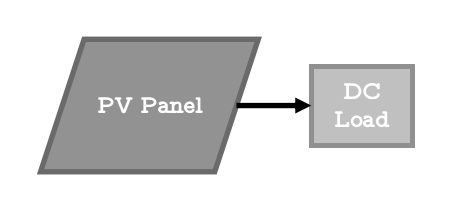
\includegraphics[width=0.6\textwidth]{unregulatedSPV.png}
\centering
\caption{Unregulated standalone SPV system with DC load (Source: \cite{Roy})}
\label{fig:unregSPV}
\end{figure}

\subsubsection{Regulated standalone PV system with DC load}
It is similar to unregulated standalone system with DC load, but the main difference between this and the previous one is that this system requires a MPPT technique, as illustrated by Fig.\ref{fig:regSPV1}. Usually system with MPPT should have battery; otherwise, extra power will be waste.

\begin{figure}[h]
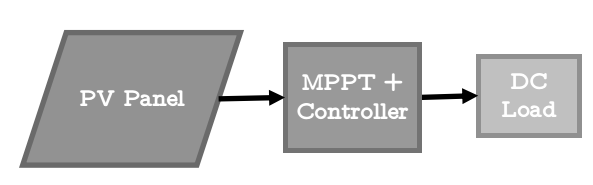
\includegraphics[width=0.8\textwidth]{regulatedSPV1.png}
\centering
\caption{Regulated standalone SPV system with DC load (Source: \cite{Roy})}
\label{fig:regSPV1}
\end{figure}

\subsubsection{Regulated standalone system with battery and DC load}
Configuration with PV array, battery, MPPT and DC load, as shown in Fig.\ref{fig:regSPV2}. Battery is used to store the extra power of PV system. A charge controller is necessary for this type of system because the useful life of the battery is less than that of the PV module. Extra charging and deep discharging can reduce the battery life \cite{Kim}. 

\begin{figure}[h]
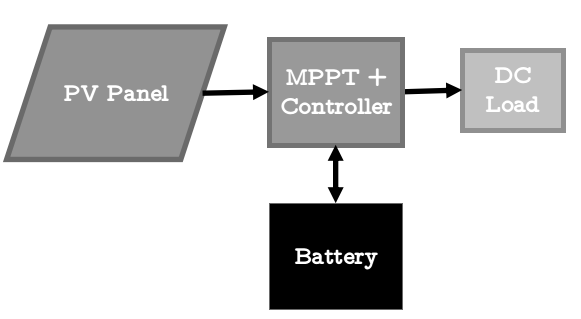
\includegraphics[width=0.8\textwidth]{regulatedSPV2.png}
\centering
\caption{Regulated standalone SPV system with battery DC load (Source: \cite{Roy})}
\label{fig:regSPV2}
\end{figure}

According to \cite{Pinho}, PV systems that are used to feed loads with low variation on the consumption can be sized to operate without the controller. That is called of self-regulated standalone PV system with battery. However, the voltage from the PV panel must be compatible with the batteries voltage. Normally, the bank of batteries are oversized related to the PV panel and to the load. The drawback is the operation of the batteries, normally overloaded or with excessive discharges (that can damage the batteries).

\subsubsection{Regulated standalone system with battery, AC load}
This system is similar to the previous one, but here AC load draws the power from PV system and, because of the AC load, an inverter (DC to AC converter) is required, as seen in Fig.\ref{fig:regSPV3}. This solution has an increase of cost because has more equipments. However, the AC availability brings the advantage of a higher number of AC appliances to use at the houses or consumer units. That configuration is the focus of the present thesis since it is the most common nowadays all over the world, when off-grid or isolated regions is the target.

\begin{figure}[h]
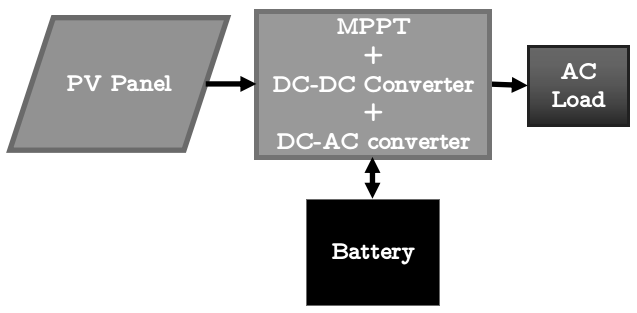
\includegraphics[width=0.8\textwidth]{regulatedSPV3.png}
\centering
\caption{Regulated standalone system with battery, AC load (Source: \cite{Roy})}
\label{fig:regSPV3}
\end{figure}

\subsection{Design and Validation of a Solar photovoltaic system}
The design and validation of a SPV system can be done by hand or with the aid of a software tool. 

In order to address different aspects of project system and systems design, there is a myriad of public domain and commercial software available for the SPV market. According to \cite{Brooks}, the capabilities of these tools range from simple solar resource and energy production estimative, to site survey and system design tools, to complex financial analysis software (with optimization). Some tools also provide support to rebate programs applications and tax incentives (specific to each country or region), while other programs and worksheets focus on the technical aspects of system sizing and design.
 
Manufacturers and integrators have yet their proprietary software to perform inverter string sizing and various system sizing and design tools, with the drawback to just include their own products among the possibilities of choice. 
In this study, the most popular tools are presented: 

\begin{itemize}
\item PVWatts 
\item SAM
\item Homer
\item RETScreen
\item Hybrid2
\end{itemize}

\subsubsection{PVWatts Calculator}
According to \cite{Freeman} and \cite{NRELDobos}, it is a web application developed by the National Renewable Energy Laboratory (NREL), which estimates the electricity production of a grid-connected roof- or ground-mounted photovoltaic system based on a few inputs. According to \cite{NRELDobos}, to use the calculator, it is necessary to provide information about the system's location, basic design parameters, and system economics. PVWatts calculates estimated values for the system's annual and monthly electricity production, and for the electricity monetary value. This tool is suitable for very preliminary studies of a potential location for a photovoltaic system that uses crystalline silicon or thin film photovoltaic modules. The production estimates that PVWatts computation do not account for many factors that are important in the design of a photovoltaic system, therefore it is necessary support of an energy expert. The calculator estimates the monthly and annual electricity production of a photovoltaic system using an hour-by-hour simulation over a period of one year. To represent the system's physical characteristics, PVWatts requires values for six inputs: System DC size; Module type; Array type; System losses; Array tilt angle; Array azimuth angle.

\subsubsection{SAM}
SAM or System Advisor Model is a software from the U.S. Department of Energy and National Renewable Energy Laboratory. According to \cite{NRELBlair} and \cite{Cameron2008}, SAM is intended to help users to determine whether the model meets their project constraints/specifications, and (also) to provide information for readers who do not plan to use the model, but want to learn about its capabilities. SAM is a performance and financial model designed to facilitate decision making for people involved in the renewable energy industry: Project managers and engineers; Financial and policy analysts; Technology developers; and Researchers. SAM makes performance predictions and cost of energy estimates for grid-connected power projects based on installation and operating costs and system design parameters that you specify as inputs to the model. Projects can be either on the customer side of the utility meter, where they buy and sell electricity at retail rates, or on the utility side of the meter, where they sell electricity at a price negotiated through a power purchase agreement. SAM is an electric power generation model and assumes that the renewable energy system delivers power either to an electric grid, or to a grid-connected building or facility to meet electric load. It does not model thermal energy systems that meet a thermal process load. As mentioned in \cite{NRELBlair}, SAM does not model isolated or off-grid power systems, and does not model systems with electricity storage batteries.

\subsubsection{HOMER}
As defined in \cite{HOMER}, actually is a set of two tools: HOMER Legacy and HOMER Pro. HOMER is an acronym for Hybrid Optimization Model for Multiple Energy Resources. HOMER Legacy is the original HOMER software version created at the National Renewable Energy Laboratory (NREL). HOMER Legacy is a free computer model that simplifies the task of evaluating design options for both off-grid and grid-connected power systems for remote, stand-alone, and distributed generation applications. HOMER's optimization and sensitivity analysis algorithms allow the user to evaluate the economic and technical feasibility of a large number of technology options. Since 2016 Homer Legacy can be found at HOMER web site, but only available for students and nonprofit organizations, as defined in \cite{HOMER}, and has not support available. At the short-time only the commercial version will remain.
 
The commercial version (paid), called HOMER Pro, as defined in \cite{Swarnkar}, is a tool for optimizing micro-grid design in all sectors, from village power and island utilities to grid-connected campuses and military bases. HOMER Pro put together three tools in one product: optimization, simulation, and sensitivity analysis. HOMER Pro provides the detailed rigor of chronological simulation and optimization in a model that is intended to be easy to use. It is adaptable to a wide variety of projects. For a village or community-scale power system, HOMER can model both the technical and economic factors involved in the project. For larger systems, HOMER can provide an overview that compares the cost and feasibility of different configurations. Chronological simulation is essential for modeling variable resources, such as solar and wind power and for combined heat and power applications, where the thermal load is variable. HOMER's sensitivity analysis helps determine the potential impact of uncertain factors such as fuel prices or wind speed on a given system. 

\subsubsection{RETScreen}
As mentioned in \cite{Pradhan}, RETScreen is a decision-support tool designed to help decision makers and energy professionals to evaluate the financial viability of renewable energy, energy efficiency, and/or co-generation projects.

RETScreen models various types of renewable energy technologies (RETs), allowing for comparisons between technology options. The software can be used to evaluate benefits from both clean energy production from power generation projects and savings through energy efficiency projects, accounting for project costs, greenhouse gas emission reductions, and financial risk. The software is freely distributed (but with restrictions to save work or print), and had three different versions:

\begin{itemize}
\item RETScreen 4 (discontinued, requires Microsoft Excel to run); 
\item RETScreen Software Suit, which includes the RETScreen 4 and a Windows-based graphical software that allows project owners to verify the ongoing energy performance of their facilities (discontinued in 2013);
\item And the actual (2016) RETScreen Expert, which allows users to evaluate energy investments over an entire project life-cycle (including benchmarking, feasibility, and performance analysis) in a fully integrated way, and within one software platform. However, this version works is only Windows-based. This version has a complete paid version, in an annual subscription way.
\end{itemize}

As described by \cite{Pradhan}, RETScreen performs a five-step standard analysis: setting and site conditions; energy model; cost analysis; emission analysis, financial analysis, sensitivity, and risk analysis. It is developed and maintained by the Government of Canada, through the CanmetENERGY Varennes Research Centre of Natural Resources; in collaboration with: NASA; Renewable Energy and Energy Efficiency Partnership (REEEP); United Nations Environment Programme (UNEP), and the Global Environment Facility (GEF). RETScreen is available in 36 languages; it is a multi-awarded tool, and includes equipment databases for components manufactured and available worldwide.

\subsubsection{Hybrid2}
The Hybrid2 software package, as described in \cite{Mills}, is a user-friendly tool to perform detailed long-term performance and economic analysis on a wide variety of hybrid power systems. Hybrid2 is a probabilistic/time series computer model, using time series data for loads, wind speed, solar insolation, and temperature; and the power system is designed or selected by the user, in order to predict the performance of the hybrid power system. Variations in wind speed and in load within each time step are factored into the performance predictions. The code does not consider short-term system fluctuations caused by system dynamics or component transients. This program is not supported anymore and according to \cite{UMASS}, probably after the user performs the free download of the tool, it will not work on Windows platforms later than Windows XP, what is a limitation.

Table \ref{table:softwares} summarizes the tools described in this paper.  Where just Hybrid2 do not have technical support; only HOMER, RETScreen and Hybrid2 perform off-grid system or battery backup analysis; all the tools perform solar photovoltaic analysis; and that only HOMER and RETScreen are complete, including economical analysis or even optimization-sensitive analysis. However, only paid version of those softwares have all the features, and they run only at Windows-based operational systems.

\begin{table}[!t]
%% increase table row spacing, adjust to taste
\renewcommand{\arraystretch}{1.3}
% if using array.sty, it might be a good idea to tweak the value of
% \extrarowheight as needed to properly center the text within the cells
\caption{Comparative coverage of reference softwares}
\label{table:softwares}
\centering
%% Some packages, such as MDW tools, offer better commands for making tables
%% than the plain LaTeX2e tabular which is used here.
\begin{tabular}{c | c | c | c | c | c}
\hline
\hline
Characteristic  & \rotatebox{90}{PVWatts} & \rotatebox{90}{SAM} & \rotatebox{90}{HOMER} & \rotatebox{90}{RETScreen } & \rotatebox{90}{Hybrid2}\\
\hline
Support & X & X & X & X &  \\
Off-grid systems &   &   & X & X & X\\
Hybrid systems &  &  & X & X & X\\
Photovoltaics & X & X & X & X & X\\
Batteries &  &  & X & X & X\\
Main technical (T) or economical (E) & T & T & E & E & T \\
Optimization &  &  & X & X &  \\
Sensitive analysis &  &  & X & X & \\
\hline
\hline
\end{tabular}
\end{table}

\subsubsection{Paper Proposal x Reference Tools}
Considering that the focus of this research is on off-grid solutions and supported tools, only HOMER and RETScreen remain for comparative. All tools need some parameters inherently from manufacturer's catalog, so the project starts with manufacturers and integrators tool to define the basic items of the project: panels, inverters, controllers, and batteries. After that, the potential solution is analyzed in another tool to validate or even optimize the solution. Therefore, that is the challenge of this work, i.e., to prove that is possible to use automated verification to validate an off-grid PV solution.

\subsection{Component models for stand-alone PV system }
The main purpose of this section is to describe the models for the elements of a standalone PV system: PV generator, battery, controller, inverter, and load. The modeling of the PV system is based on modular blocks, as illustrated in Fig.\ref{fig:blockdiagram}, from \cite{Hansen}. The modular structure facilitates the modeling of the other system structures and replacing of elements as, for instance, a DC load instead of an AC load. 

\begin{figure}[h]
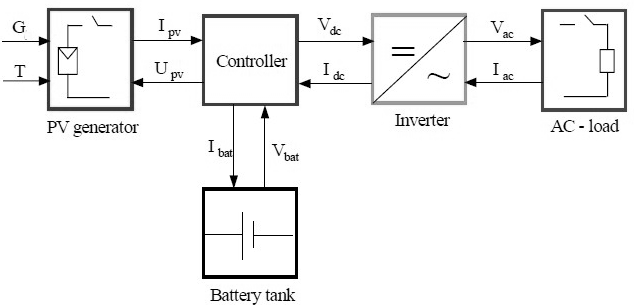
\includegraphics[width=0.95\textwidth]{blockdiagramPVS}
\centering
\caption{Block diagram for the stand-alone PV system (Source: \cite{Hansen})}
\label{fig:blockdiagram}
\end{figure}

In the literature, there are several mathematical models available for each component of stand-alone PV systems. In this section, the mathematical model for each component of PV system is presented. 

\subsubsection{PV generator (cell, module, array) }
A photovoltaic PV generator is the whole assembly of solar cells, connections, protective parts, and supports. In the present modeling, the focus is only on cell/module/array.
 
The basic element of a PV System is the PV cell, also called a Solar Cell. A PV / Solar Cell is a semiconductor device that can convert solar energy into DC electricity. The semiconductor materials (usually silicon), which are specially treated to form an electric field, positive on one side (backside) and negative on the other (towards the sun). When solar energy (photons) hits the solar cell, electrons are knocked loose from the atoms in the semiconductor material, creating electron-hole pairs \cite{Lorenzo}. If electrical conductors are attached to the positive and negative sides, forming an electrical circuit, the electrons are captured in the form of electric current $ I_{ph} $ (photocurrent).
 
To increase their utility, a number of individual PV cells are interconnected together in a sealed, weatherproof package called Panel (or Module). For instance, a 12 V Panel will have 36 cells connected in series and a 24 V Panel will have 72 PV cells connected in series. In addition, to achieve the desired voltage and current, modules are wired in series and parallel into what is called a PV Array, as shown in Fig.\ref{fig:celmodarray}. The flexibility of the modular PV system allows designers to create PV systems that can meet a wide variety of electrical demands. 

\begin{figure}[h]
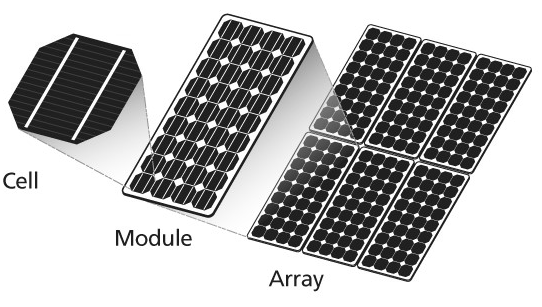
\includegraphics[width=0.95\textwidth]{celmodarray}
\centering
\caption{PV cell, module and array (Source: \cite{SamlexSolar})}
\label{fig:celmodarray}
\end{figure}

The PV modules are generally rated under standard test conditions (STC), which leads to the following specification by the manufacturers:  solar radiation of 1000 W/m$^{2}$, cell temperature of 25$^{o}$C, and solar spectrum of 1.5. The parameters required for the input of the PV modules are relying on the meteorological conditions of the area to be serviced by photovoltaic solution. However, the climatic conditions are unpredictable due to the random nature of their occurrence \cite{Jakhrani}.
 
These uncertainties lead to either over- or underestimation of energy yield from PV modules. An overestimation up to 40\% was reported as compared to the rated power output of PV modules \cite{Durisch}. The growing demand of photovoltaics technologies led to research in the various aspects of its components from cell technology to the modeling, size optimization, and system performance \cite{Rajanna}, \cite{Badejani}; \cite{Yatimi}, \cite{Ferrari}, \cite{Saloux}, \cite{Hasan}, \cite{King}, \cite{Mellit}. Modeling PV modules is one of the major components responsible for proper functioning of PV systems. However, the estimation of models is affected by various intrinsic and extrinsic factors, which ultimately influence the behavior of current and voltage. Therefore, perfect modeling is essential to estimate the performance of PV modules in different environmental conditions \cite{Jakhrani}.
 
Modeling provides the ways to understand the current, voltage, and power relationships of PV systems.
  
The performance of photovoltaic systems (solar cell/panels), that is, the output current/voltage curve ($I-V$ curve), is usually studied using an equivalent circuit model. This equivalent circuit consists of a current source with one or two diodes connected in parallel, and up to two resistors, one connected in parallel and the other one in series, to take into account energy losses in this model \cite{Cubas}. Based on these electronic components, four basic configurations are normally used when studying photovoltaic systems, as shown by Fig. \ref{fig:equivckt}. 

\begin{figure}[h]
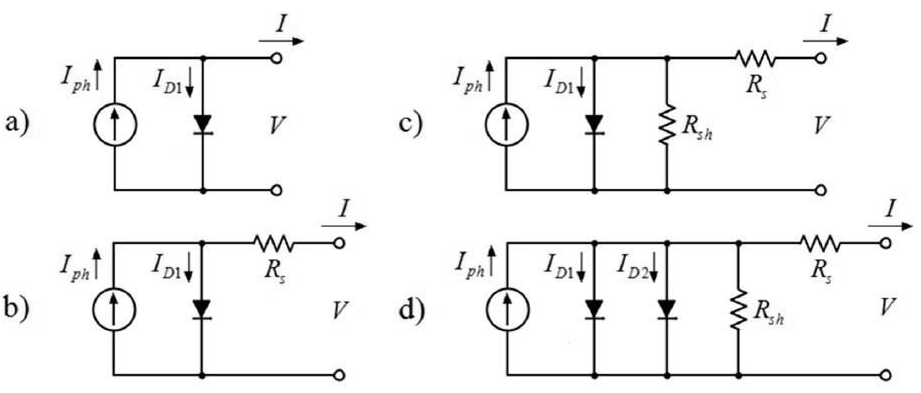
\includegraphics[width=0.95\textwidth]{equivckt}
\centering
\caption{Four different equivalent circuit models: (a) 1-diode; (b) 1-diode/1-resistor; (c) 1-diode/2-resistor; (d) 2-diode/2-resistor (Source: \cite{Cubas})}
\label{fig:equivckt}
\end{figure}
 
The 1-diode model, whose equation to relate the output current, $I$, to the output voltage, $V$, is described in Equation \ref{eq:1diodemodel}. 

\begin{equation}
\label{eq:1diodemodel}
I = I_{ph}-I_{D1}=I_{ph}-I_{0}\left[ exp \left( \dfrac{V}{NaV_{T}} \right)  \right] 
\end{equation}

Where:
\begin{itemize}
\item $I_{ph}$ is the photocurrent delivered by the constant current source; 
\item $ I_{0} $ is the reverse saturation current corresponding to the diode; 
\item $ N $ is the number of series-connected cells in the photovoltaic system to be analyzed;
	\begin{itemize}
	\item $ N=1 $ in a single cell configuration. 	
	\end{itemize}	  
\item $ a $ is the ideality factor (or quality factor) that takes into account the deviation of the diodes from the Shockley diffusion theory; 
	\begin{itemize}
	\item $a=1$ for ideal diodes and between $ 1 $ and $ 2 $ for real diodes. 	
	\end{itemize}
\item $V_{T}$ is the thermal voltage ($ V_{T}=k_{B}T/q $);
	\begin{itemize}
	\item $ k_{B} $ is the Boltzmann constant ($ 1.3806503\times10^{-23}J $); 
	\item $ T $ the temperature of the p-n junction (or cell temperature) expressed in Kelvin; 
	\item $ q $ is absolute value of the electron's charge ($ -1.60217646\times10^{-19}C $).	
	\end{itemize}	 
\end{itemize}


This model has only three unknown parameters ($ I_{ph}$, $I_{0}$, and $a $), and it assumes that the series resistance is $ zero $ and shunt resistance is $ infinite $ and, thus, both of these parameters are ignored.
 
The 1-diode/1-resistor model, is described by Equation \ref{eq:1d1rmodel}. 

\begin{equation}
\label{eq:1d1rmodel}
I =I_{ph}-I_{0}\left[ exp \left( \dfrac{V+IR_{s}}{NaV_{T}} \right) -1 \right] 
\end{equation}

Where $R_{s}$ is the series resistor.

At this model, there are four unknown parameters ($ I_{ph}$, $I_{0}$, $ R_{s} $, and $ a $), and it assumes shunt resistance as $ infinite $.

The 1-diode/2-resistor model, is described by Equation \ref{eq:1d2rmodel}. 

\begin{equation}
\label{eq:1d2rmodel}
I =I_{ph}-I_{0}\left[ exp \left( \dfrac{V+IR_{s}}{NaV_{T}} \right) -1 \right] - \dfrac{V+IR_{s}}{R_{sh}}
\end{equation}

Where $R_{sh}$ is the shunt resistor.

At this model, there are five unknown parameters ($ I_{ph}$, $I_{0}$, $ R_{s} $, $ R_{sh} $, and $ a $).

And the 2-diode/2-resistor model, is described by Equation \ref{eq:2d2rmodel}. 

\begin{equation}
\label{eq:2d2rmodel}
I =I_{ph}-I_{01}\left[ exp \left( \dfrac{V+IR_{s}}{Na_{1}V_{T}} \right) -1 \right] - I_{02}\left[ exp \left( \dfrac{V+IR_{s}}{Na_{2}V_{T}} \right) -1 \right] - \dfrac{V+IR_{s}}{R_{sh}}
\end{equation}

This model has six unknown parameters with two exponential terms. 
Briefly, both single and double diode models require the knowledge of all unknown parameters, which is usually not provided by manufacturers. Nevertheless, the current-voltage equation is a transcendental expression \cite{Jakhrani}.  

However, regardless of the adopted model, the parameters of the equations must be estimated to adapt the corresponding model to the real behavior of the solar cell/panel. 

For that reason, researchers gradually focused on searching out the approximate methods for the calculation of unknown parameters and walked through three different paths. The analytical methods give exact solutions by means of algebraic equations, as done by \cite{Cubas} and \cite{Brano}. However, due to implicit nature and nonlinearity of PV cell or module characteristics, it is hard to find out the analytical solution of all unknown parameters, as described by \cite{Hasan}. Thus, numerical methods such as Newton-Raphson method or Levenberg-Marquardt algorithm were preferred, as described by \cite{Mellit}. This happens because numerical methods give approximate solution of the nonlinear problems without searching for exact solutions. However, numerical methods are time consuming and need long term time series data, which is not available in developing countries. \cite{Jakhrani} did a mixed methodology using analytical and numerical steps together.  \cite{Shenawy} create a method to discover the unknown parameters of the PV panels through experimentation (essays). And \cite{Tian} did a mix of analytical and experimental methodology to get the unknown parameters, but samples of the PV modules are necessary to perform some essays, when we use experimental technique. 

Therefore, a wide variety of models exists for estimation of power output of PV modules (and $I-V$ or $P-V$ curves). However, the present work will rely on the simplified model of 1-diode, that was shown by \cite{Saloux} that has a small error rate, between 0.03\% and 4.68\% from selected PV panels tested. In addition, this mathematical modeling has the advantage of being an explicit model, which does not use iterative numerical calculation. 


\subsubsection{Proposed PV Panel Model}
With the proposed model, an explicit set of equations is derivate from the ideal PV model given by Equation \ref{eq:1d1rmodel}.

A single-diode without series and shunt resistances is considered. Equation 1 is used to write down expressions for currents and voltages at each key point shown in Fig. \ref{fig:ivcurve}.

\begin{figure}[h]
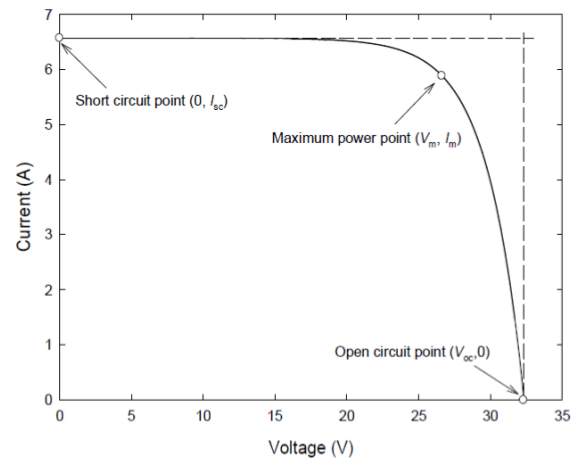
\includegraphics[width=0.90\textwidth]{ivcurve}
\centering
\caption{$ I-V $ characteristic curve of an ideal PV cell (Source: \cite{Saloux})}
\label{fig:ivcurve}
\end{figure}

Hence, the short-circuit current, the open-circuit voltage, the maximum power voltage and current are written as defined by \cite{Saloux} and shown from Equations \ref{eq:Isc} to \ref{eq:Im}.

\begin{equation}
\label{eq:Isc}
I_{sc}=I_{ph}\vert_{V=0}
\end{equation}

\begin{equation}
\label{eq:Voc}
V_{oc}=\dfrac{aNk_{B}T}{q}ln\left( 1+\dfrac{I_{sc}}{I_{0}} \right) 
\end{equation}

\begin{equation}
\label{eq:exp}
exp\left( \dfrac{qV_{oc}}{aNk_{B}T} \right) = \left(1+\dfrac{qV_{m}}{aNk_{B}T} \right) exp \left( \dfrac{qV_{m}}{aNk_{B}T} \right) 
\end{equation}

\begin{equation}
\label{eq:Im}
I_{m} =I_{ph}-I_{0}\left[ exp \left( \dfrac{qV_{m}}{aNk_{B}T} \right) -1 \right] 
\end{equation}

Equation \ref{eq:exp} is not explicit with the PV key parameters, therefore need to be rewritten in a different way. A PV cell has a hybrid behavior, i.e., a current-source at the short-circuit point and voltage-source at the open-circuit point \cite{Saloux}. These two regions are characterized by two asymptotes of the $ I-V $ curve in Fig. \ref{fig:ivcurve}, where the transition is a compromise between both behaviors. It is interesting to observe that the maximum power point corresponds to a trade-off condition, where the current is still high enough before it starts decreasing with increasing the output voltage (Fig. \ref{fig:ivcurve}).

Based on this, the tangent of the I-V curve can be used to evaluate the transition between current- to voltage-source controlled regions; this operation yields Equation \ref{eq:didv}.

\begin{equation}
\label{eq:didv}
\dfrac{dI}{dV}=-\dfrac{qI_{0}}{aNk_{B}T}exp \left( \dfrac{qV}{aNk_{B}T}  \right) 
\end{equation}

The derivative of Equation \ref{eq:didv} is used to calculate the output voltage that corresponds to the maximum power operation condition of the cell. Therefore, the Equation \ref{eq:Vmderiv} is generated.

\begin{equation}
\label{eq:Vmderiv}
V_{m}=\dfrac{aNk_{B}T}{q} ln \left( -\dfrac{qNk_{B}T}{qI_{0}} \left( \dfrac{dI}{dV}  \right)_{V_{m}}   \right) 
\end{equation}

It is evident that Equation \ref{eq:Vmderiv} requires an expression of the derivative of the current with voltage evaluated at the maximum power point. The fact that the maximum power corresponds to an extreme, the variation of the maximum output power with voltage is relatively small, i.e., a change on $ V_{m} $ has a relatively small effect on the maximum power of the cell \cite{Saloux}. Consequently, considering the asymptotic behavior of the $I-V$ curve at short- and open-circuit conditions, the derivative required by Equation 10 can be calculated as shown in Equation \ref{eq:dIdV_Vm}.

\begin{equation}
\label{eq:dIdV_Vm}
\dfrac{dI}{dV}\vert_{V_{m}} \cong -\dfrac{0-I_{sc}}{V_{oc}-0}=\dfrac{I_{sc}}{V_{oc}}
\end{equation}

Replacing the Equation \ref{eq:dIdV_Vm} into Equations \ref{eq:Vmderiv} and \ref{eq:Im}, the voltage and the current at the maximum power point and consequently the maximum output power, are expressed by Equations \ref{eq:Vmfinal}, \ref{eq:Imfinal}, and \ref{eq:Pm} ($ P_{m}=V_{m}I_{m} $). These equations are used to calculate the key cell parameters at the maximum power point as function cell temperature and parameters from the manufacturer's data-sheet.

\begin{equation}
\label{eq:Vmfinal}
V_{m}=\dfrac{aNk_{B}T}{q} ln \left( \dfrac{aNk_{B}T}{qI_{0}} \dfrac{I_{sc}}{V_{oc}}  \right) 
\end{equation}

\begin{equation}
\label{eq:Imfinal}
I_{m} = I_{ph} + I_{0} - \dfrac{aNk_{B}T}{q} \left( \dfrac{I_{sc}}{V_{oc}} \right)  
\end{equation}

\begin{equation}
\label{eq:Pm}
P_{m} = \left[ \dfrac{aNk_{B}T}{q} ln \left( \dfrac{aNk_{B}T}{qI_{0}} \dfrac{I_{sc}}{V_{oc}}  \right) \right] \times \left[ I_{ph} + I_{0} - \dfrac{aNk_{B}T}{q} \left( \dfrac{I_{sc}}{V_{oc}} \right)  \right] 
\end{equation}


However, the photocurrent delivered by the constant current source ($ I_{ph} $) or even the reverse saturation current ($ I_{0} $) are not given by PV manufacturers. Therefore, Equation \ref{eq:Iph} is used to calculate the photocurrent as function of irradiance and temperature \cite{Villalva}.

\begin{equation}
\label{eq:Iph}
I_{ph}=\dfrac{G}{G_{ref}} \left[ I_{ph,ref} + \mu_{I} \left( T-T_{ref} \right)    \right] 
\end{equation}

Where the reference state (STC) of the cell is given by the solar irradiance $ G_{ref}=1000 W/m^{2} $, and the temperature $ T_{ref}=298.15 K (=25^{o}C) $.

In Equation \ref{eq:Iph}, $ \mu_{I} $ is the short-circuit current temperature coefficient ($A/K$) and corresponds to the photocurrent obtained from a given PV cell working at (STC or standard test conditions) reference conditions (provided by PV manufacturers). $ I_{ph,ref} $ can also be approximated to the reference short-circuit current that is provided by PV manufacturers ($ I_{sc,ref} $) as shown by \cite{Jakhrani}.

The cell temperature ($ T $) can be obtained from \cite{Ross} and is shown in Equation \ref{eq:Tcell}.

\begin{equation}
\label{eq:Tcell}
T = T_{air} + \dfrac{NOCT-20}{800}G
\end{equation}

Where $ T_{air} $ is the ambient temperature, $NOCT$ is the nominal operating cell temperature (in $^{o}$C) that is found at the PV manufacturer's data-sheet, and $G$ is the solar irradiance ($ W/m^{2} $) of the place where the PV system is deployed.

Furthermore, \cite{Villalva} have proposed a relationship, which allows the saturation current ($ I_{0} $) to be expressed as a function of the cell temperature. In this study, this relation is explicitly written based on cell open-circuit conditions using the short-circuit current temperature coefficient as well as the open-circuit voltage temperature coefficient (Equation \ref{eq:I0}).

\begin{equation}
\label{eq:I0}
I_{0} = \dfrac{I_{sc,ref} + \mu_{I}(T - T_{ref})}{exp \left[ \dfrac{q(V_{oc,ref} + \mu_{V} (T - T_{ref}))}{aNk_{B}T}    \right] -1}
\end{equation}

Where $ V_{oc,ref} $ is the reference open-circuit voltage, and $ \mu_{V} $ is an open-circuit voltage temperature coefficient ($ V/K $).

The ideality (or quality) factor of the diode $ a $, which is usually considered as a constant \cite{Villalva}, is determined in the reference state. Using the maximum power point current equation (Equation \ref{eq:Pm}) and the saturation current in the reference temperature given by Equation \ref{eq:I0}, the diode quality coefficient is determined by Equation \ref{eq:a}.

\begin{equation}
\label{eq:a}
a = \dfrac{q(V_{m,ref}-V_{oc,ref})}{Nk_{B}T} \dfrac{1}{ln \left( 1 - \dfrac{I_{m,ref}}{I_{sc,ref}}  \right) }
\end{equation}

Where $ V_{mref} $, $ V_{oc,ref} $, $ I_{m,ref} $, and $ I_{sc,ref} $ are key cell values obtained under both actual cell temperature and solar irradiance conditions, usually provided by manufacturers.

The model is now completely determined; it requires the actual cell temperature (or the air temperature), the actual solar irradiance and common data provided by manufacturers.

If the PV cells are in parallel, then there is a parallel array. Therefore, there will be a change at the $ I_{ph} $ and $ I_{0} $and the resulting current is given by Equation \ref{eq:Iarray}, as demonstrated in \cite{Saloux}.

\begin{equation}
\label{eq:Iarray}
I_{array} = (N_{cells in parallel})(I_{one cell})
\end{equation}

Where $ I_{one cell} $ is the current from Equation \ref{eq:Imfinal}.

In addition, if the panels are in series, the current do not change but the total voltage is the sum of the each panel's voltage.

\begin{equation}
\label{eq:Varray}
V_{array} = (N_{cells in series})(V_{one panel})
\end{equation}

Where $ V_{one panel} $ is the voltage from Equation \ref{eq:Vmfinal}.

Besides the model verification, there is the prior stage of project sizing check, which is simple, based on manufacturer's data and information from the sizing and the site. 

First is necessary to correct the energy consumption that was estimated to the load ($E_{consumption}$). That is done by Equation \ref{eq:Ecorrected}, according \cite{Pinho}. Where the efficiency of batteries ($\eta_{b}$), controller ($\eta_{c}$), and the inverter ($\eta_{i}$) are considered.

\begin{equation}
\label{eq:Ecorrected}
E_{corrected} = \dfrac{E_{consumption}}{ \eta_{b} \eta_{c} \eta_{i} }
\end{equation}

The total minimum number of solar panels necessary($ N_{TPmin} $) is calculated by Equation \ref{eq:NTPmin}, and the check is done with the Equation \ref{eq:NTP}, where the sized number of panels ($ N_{TP} $) must be greater than the result from Equation \ref{eq:NTPmin}.

\begin{equation}
\label{eq:NTPmin}
N_{TPmin} = \dfrac{E_{corrected}}{E_{p}}
\end{equation}

\begin{equation}
\label{eq:NTP}
N_{TP} \geq N_{TPmin}
\end{equation}

Particularly, the total number of panels is series ($ N_{PSmin} $) and parallel ($ N_{PPmin} $) are given by the Equations \ref{eq:NPSmin} and \ref{eq:NPPmin}, respectively. With the check did by Equations \ref{eq:NPS} and \ref{eq:NPP}. $ V_{system} $ is the DC voltage of the bus, and is a design decision (normally 12, 24 or 48 V).

\begin{equation}
\label{eq:NPSmin}
N_{PSmin} = \dfrac{V_{system}}{V_{m,ref}}
\end{equation}

\begin{equation}
\label{eq:NPPmin}
N_{PPmin} = \dfrac{N_{TPmin}}{N_{PSmin}}
\end{equation}

\begin{equation}
\label{eq:NPS}
N_{PS} \geq N_{PSmin}
\end{equation}

\begin{equation}
\label{eq:NPP}
N_{PP} \geq N_{PPmin}
\end{equation}


\subsubsection{The Battery Storage Model }
Because of the fluctuating nature of the output delivered by the PV arrays, batteries are necessary in a PV system. Thus, during the hours of sunshine, the PV system feeds directly the load and the excess electrical energy is stored in the battery. During the night, or during a period with low solar irradiation, energy is supplied to the load from the battery \cite{Mellit}.
  
Several models have been presented in the literature. However, regardless of the model, normally the following parameters are required: 

\begin{itemize}
\item Nominal capacity ($ q_{m} $), is the number of Ampère-hours ($ Ah $) that can maximally be extracted from the battery, under predetermined discharge conditions.
\item State of charge ($ SOC $), is the ratio between the present capacity and the nominal capacity, i.e., $ SOC = q/q_{max} $. Obviously $ 0<SOC<1 $. If $ SOC=1 $, then the battery is totally charged; and if $ SOC=0 $, the battery is fully discharged
\item Charge (or discharge) regime.This parameter reflects the relationship between the nominal capacity of a battery and the current at which it is charged (or discharged). It is expressed in hours: for instance, discharge regime is 30h for a battery of 150 Ah that is discharged at 5A.
\item Efficiency ($\eta_{b}$), is the ratio of the charge extracted during discharge divided by the amount of the charge needed to restore the initial state of charging or discharging current. 
\item Lifetime, is the number of charge/discharge cycles the battery can sustain before losing 20\% of its nominal capacity.
\end{itemize}

The merit of a stand-alone PV system is evaluated in terms of the reliability of the electricity supply to the load and in terms of the long-term efficiency of the components. The battery efficiency was described in this section, and the liability is quantified by the concept of loss of load probability (LLP). LLP is defined as the ratio between the Ampere-hour deficit and the Ampere-hour demand, both with respect to the load, over a long period of time \cite{Copetti}. 

In general, the battery models view the battery as a voltage source $ E $ in series with an internal resistance $ R_{0} $, as shown in Fig. \ref{fig:batteryckt}. 

\begin{figure}[h]
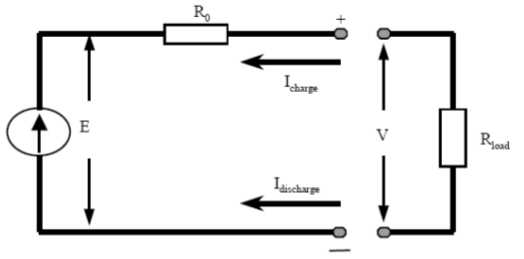
\includegraphics[width=0.7\textwidth]{batteryckt}
\centering
\caption{Schematic diagram of the battery (Source: \cite{Hansen})}
\label{fig:batteryckt}
\end{figure}


The terminal voltage of the battery can be expressed in terms of its open circuit voltage and the voltage across the internal resistance of the battery \cite{Sukamongkol}, as shown by Equation 31.  

Where $ V_{b} $ is the battery terminal voltage, $ E_{oc} $ is the battery circuit voltage, $ I_{b} $ is the battery current, and $ R_{b} $ is the internal resistance of the battery.

The battery model, which describes the relationship between the voltage, current and the state of charge, can be found in \cite{Copetti}, \cite{Manwell93}, and \cite{Manwell94}.  

The Kinetic Battery Model (KiBaM) of Manwell and McGowen \cite{Manwell93} was developed at the University of Massachusetts to predict the performance of the battery, based on manufacturer's data. However, it uses some data extracted from tested batteries in laboratory. Therefore is not suitable to this study. 

Most of the created models were used to simulate and optimize PV storage system based on lead-acid batteries. That kind of battery is the most common used batteries in PV application, owing to their relative low cost and wide availability \cite{Copetti}. 

Here, the model adopted is the based on \cite{Copetti}, who uses manufacturer's data and allows finding relations among voltage, current, state of charge and temperature. 

The discharge voltage equation is shown in Equation \ref{eq:bat_Vd}. The first term represents the voltage variation with the state of charge ($ SOC $), i.e., the electrolyte concentration, and the second is the variation due to internal resistance variation.

\begin{equation}
\label{eq:bat_Vd}
V_{d} = \left[ 2.085-0.12(1-SOC) \right] - \dfrac{I}{C_{10}} \left( \dfrac{4}{1+I^{1.3}} + \dfrac{0.27}{SOC^{1.5}}+0.02 \right) (1-0.007 \Delta T)
\end{equation}

Where $ C_{10} $ means 10h of rated capacity, which is standard on the manufacturer's data-sheet, $ \Delta T $ is temperature variation ($ \Delta T=T-T_{ref} $, $ T_{ref}=25^{o}C $, $ SOC $ indicates how much electric charge is stored in the cell at given time, defined by Equation \ref{eq:SOCbat}.

\begin{equation}
\label{eq:SOCbat}
SOC = \left( 1 - \dfrac{Q}{C} \right) 
\end{equation}

Where $ Q $ is the charge delivered at the time of interest ($ Q=It $), and C is the battery capacity.

The ratio between $ Q $ and $ C $ represents the depth of discharge ($ DOD $) or the farction of discharge, i.e., $ DOC=1-SOC $.

The efficiency of the battery discharge is assumed to be 100\%, according \cite{Copetti}; however, the total amount of useful charge available during discharge is limited by the current rate and temperature given by Equation \ref{eq:CC10}. This equation, called of capacity, is normalized with respect to discharge current corresponding to $ C_{10} $ rated capacity ($ I_{10} $).

\begin{equation}
\label{eq:CC10}
\dfrac{C}{C_{10}} = \dfrac{1.67}{1+0.67 \left( \dfrac{I}{I_{10}} \right)^{0.9} }(1+0.005 \Delta T)
\end{equation}

Note that when the discharge current tends to zero at 25$^{o}$C, the maximum capacity that can be removed is about 67\% over the capacity.

For the charging process, however, the parameters are presented in Equation \ref{eq:Vcbat}.

\begin{equation}
\label{eq:Vcbat}
V_{c} = [2+0.16SOC]+ \dfrac{I}{C_{10}} \left( \dfrac{6}{1+I^{0.86}} + \dfrac{0.48}{(1-SOC)^{1.2}} + 0.036  \right) (1-0.025 \Delta T)
\end{equation}

SOC can be calculated easily at any point during the discharge period; however, during recharge it is much more difficult \cite{Copetti}.

Generally, the efficient region is where $ SOC $ is below $ 0.7 $ and $ V_{c} $ is less than $2.3 V$ per cell. The efficiency drops to zero at full charge and the function that represents the charge efficiency ($ \eta_{c} $) variation with state of charge and current rate is given in Equation \ref{eq:efficcharge}.

\begin{equation}
\label{eq:efficcharge}
\eta_{c} = 1 - exp \left[ \dfrac{20.73}{\dfrac{I}{I_{10}}+0.55} (SOC-1) \right] 
\end{equation}

\cite{Copetti} show that, during overcharge, gassing occur and tests demonstrated that the final charge voltage ($ V_{ec} $) increases with the current intensity and with the decreasing of the temperature (Equation \ref{eq:Vec}). It was created a function for the gassing voltage as well, as shown in Equation \ref{eq:Vg}. In addition, the overcharge phenomenon can be represented by Equation \ref{eq:Voverc}.

\begin{equation}
\label{eq:Vec}
V_{ec} = \left[ 2.45 + 2.011 ln \left( 1+\dfrac{I}{C_{10}} \right)  \right] (1-0.002 \Delta T)
\end{equation}

\begin{equation}
\label{eq:Vg}
V_{g} = \left[ 2.24 + 1.97 ln \left( 1+\dfrac{I}{C_{10}} \right)  \right] (1-0.002 \Delta T)
\end{equation}

\begin{equation}
\label{eq:Voverc}
V_{c} = V_{g} + (V_{ec} - V_{g}) \left[ 1- exp \left( \dfrac{Ah_{restored}-0.95C}{I\tau}  \right)    \right] 
\end{equation}

Where $ Ah_{restored} $ represents the Ampère-hour stored in the battery with regard to the battery capacity ($ C $) during this hour.

The function assumes that 95\% of the capacity was already restored at the start of overcharge.

The time constant of the phenomenon ($ \tau $) is reversely proportional to the charge intensity and can be written by Equation \ref{eq:tau}.

\begin{equation}
\label{eq:tau}
\tau = \dfrac{17.3}{1+852 \left( \dfrac{I}{C_{10}} \right) ^{1.67} }
\end{equation}

Therefore, to model the voltage ($ V_{c} $) evolution of the battery, equation \ref{eq:Vcbat} can be used up the start of gassing ($ V_{c} \leq V_{g} $). And during overcharging ($ V_{c} > V_{g} $), Equation \ref{eq:Voverc} can be used until a constant final voltage ($ V_{ec} $) is reached.

The storage capacity of the battery can be calculated using Equation \ref{eq:stor}, as defined in \cite{Wenham}.

\begin{equation}
\label{eq:stor}
Storage capacity = \dfrac{N_{C}E_{load}}{DOD \eta _{b}}
\end{equation}

Where $ DOD $ is the maximum possible depth of battery discharge, $ E_{load} $ is the average energy consumed by the load, $ N_{C} $ is the largest number of continuous cloudy days of the area, and $ \eta_{b} $ is the efficiency of the battery.

As an example of this formula application, as shown by \cite{Abdulateef}, considering that an off-grid PV system is intended to supply $1.5 kW/48 V$ for 24 hours ($=36 kWh$); The largest number of continuous cloudy days in the selected site is about 1 day; For a maximum depth of discharge for the battery $DOD$ of $0.8$ and battery efficiency $80\%$.

Then the storage capacity using Equation \ref{eq:stor} becomes $56.3 kWh$. Since the selected DC bus voltage is $48 V$, then the required Ampere-hours of the battery is $1173 Ah$ ($56.3 kWh/48$). If a single battery of 12 V and 350 Ah is considered, then four batteries are connected in series ($4 \times 350 Ah = 1400 Ah$).

At this research, it was considered a simplified model for charging (Equation \ref{eq:charge}) and discharging (Equation \ref{eq:discharge}) of the batteries, even considering that the process is not linear and depends on the temperature. The equations are used to update the $SOC$ of the batteries, and have the number of hours ($ Num_{h} $) as a variable. There is a factor (1.15) which is present at the charging equation, and is necessary to express that during the charging process is usual to reach 115\% of the battery capacity

\begin{equation}
\label{eq:charge}
SOC_{charge} = SOC_{previous} + \dfrac{100*Pm*Num_{h}}{V_{system}*capacity*N_{BP}*1.15}
\end{equation}

\begin{equation}
\label{eq:discharge}
SOC_{discharge} = SOC_{previous} - \dfrac{100*I_{drained}*Num_{h}}{capacity}
\end{equation}


Besides the model verification, there is also the prior stage of project sizing check, as did to the solar panel. First is necessary to define the total capacity of the battery bank, as shown by Equation \ref{eq:Cbank}.

\begin{equation}
\label{eq:Cbank}
C_{bank} = \dfrac{E_{corrected} \times autonomy}{V_{system} \times DOD}
\end{equation}

The variable $ autonomy $ is a design definition and normally has a value ranging from 6 to 48h. The other variables were discussed previously.

Following, is done the total (minimum) number of batteries, as show by Equation \ref{eq:Nbtotal}. Moreover, the Equation \ref{eq:batcheck} perform the final sizing check, considering the number of batteries in series ($ N_{BS} $) and the number of batteries in parallel ($ N_{BP} $) that were established to the project.

\begin{equation}
\label{eq:Nbtotal}
N_{B}total = N_{BS}min \times N_{BP}min = \dfrac{V_{system}}{V_{bat}} \times \dfrac{C_{bank}}{C_{20}}
\end{equation}

\begin{equation}
\label{eq:batcheck}
\left( N_{BS} \times  N_{BP} \right) \geq N_{B}total
\end{equation}

\subsubsection{Controller Model}
Depending on the literature, the controller can receive different names: controller \cite{Hansen}, charge controller \cite{Mahanta} and \cite{Chauhan}, regulator \cite{Mellit}, DC-DC converter with MPPT and switch \cite{Dhanowa}, \cite{Yatimi}, \cite{Abdulateef}, \cite{Roy}. However, in this study, in order to simplify, the term used is controller. 

The controller is a set of items (DC-DC converter, a MPPT and switches) and can be defined as the responsible to manage the energy flow to PV system, batteries and loads by collecting information on the battery voltage and knowing the maximum and minimum values acceptable for the battery voltage. According to \cite{Pinho}, controllers aim to protect the battery (or batteries) against the excessive charge and discharge, improving its lifetime. 

As defined by \cite{Hansen} and \cite{Mellit}, all power systems must include a control strategy, which describes the interactions between its components. The use of battery as a storage form implies thus the presence of a charge controller. 

In general, there are two main operating modes for the controller: normal operating condition, when the battery voltage fluctuates between maximum and minimum voltages; and overcharge or over-discharge conditions, which occur when the battery voltage reaches some critical values. 

In \cite{Mellit} was established that the controller allows the management of energy between the load and the battery. The input signals for regulator model are the battery current ($ I_{br} $), PV generator's voltage ($ V_{PV} $), PV generator's current ($ I_{PV} $), and battery voltage ($ V_{b} $). The outputs are battery ($ I_{rb} $) current and used current ($ I_{u} $). 

According \cite{Hansen}, to protect the battery against an excessive charge, the PV arrays are disconnected from the system, when the terminal voltage increases above a certain threshold $ V_{max \textunderscore off} $ and when the current required by the load is less than the current delivered by the PV arrays. PV arrays are connected again when the terminal voltage decreases below a certain value $ V_{max \textunderscore on} $. This can be done by using a switch with a hysteresis cycle, as illustrated in Fig. \ref{fig:controllerover}. 

\begin{figure}[h]
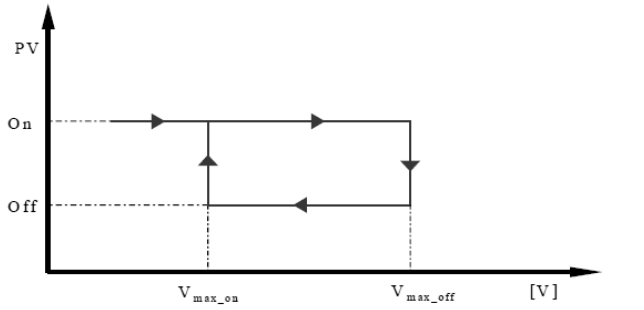
\includegraphics[width=0.7\textwidth]{controllerover}
\centering
\caption{Operating principle of an overcharge protector (Source: \cite{Hansen})}
\label{fig:controllerover}
\end{figure}

To protect the battery against excessive discharge, the load is disconnected when the terminal voltage falls below a certain threshold i and when the current required by the load is larger than the current delivered by the PV arrays \cite{Hansen}. The load is reconnected to the system, when the terminal voltage is above a certain value i, using a switch with a hysteresis cycle, as shown in Fig. \ref{fig:controllerdisc}. 

\begin{figure}[h]
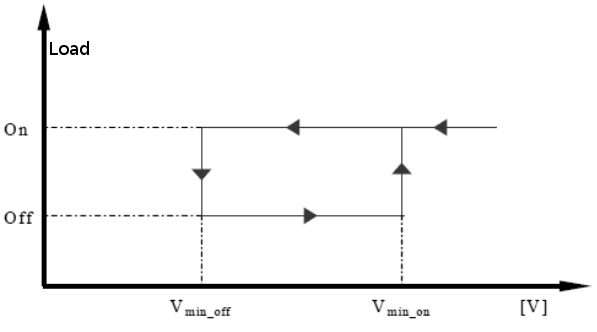
\includegraphics[width=0.7\textwidth]{controllerdisc}
\centering
\caption{Operating principle of a discharge protector (Source: \cite{Hansen})}
\label{fig:controllerdisc}
\end{figure}

According to \cite{Lorenzo}, the switches may either be electromechanical (relay, contactors, etc.) or solid state (bipolar transistors, MOSFET's, etc.). 

The steps in the modeling of the controller process are summarized in Table \ref{table:controller}.

\begin{table}[!t]
%% increase table row spacing, adjust to taste
\renewcommand{\arraystretch}{1.3}
% if using array.sty, it might be a good idea to tweak the value of
% \extrarowheight as needed to properly center the text within the cells
\caption{Summary of the controller process (Source: \cite{Hansen})}
\label{table:controller}
\centering
%% Some packages, such as MDW tools, offer better commands for making tables
%% than the plain LaTeX2e tabular which is used here.
\begin{tabular}{c | c | c }
\hline
\hline
Step  & Constraint & Command\\
\hline
\hline
(1) & \makecell{If $V > V_{max \textunderscore off}$ and $I_{load} < I_{pv}$} & \makecell{Disconnect PV array from the system}\\
\hline
(2) & \makecell{If command (1) is done and $V < V_{max \textunderscore on}$} & \makecell{Reconnect PV array to the system}\\
\hline
(3) & \makecell{If $V < V_{min \textunderscore off}$ and $I_{load} > I_{pv}$} & \makecell{Disconnect the load from the system}\\
\hline
(4) & \makecell{If command (3) is done and $V > V_{min \textunderscore on}$} & \makecell{Reconnect the load to the system}\\
\hline
\hline
\end{tabular}
\end{table}

Regarding the DC-DC converter, the most basic idea is that the power is converted while altering the current and voltage. 

As shown in \cite{Abdulateef}, the DC-DC converter is used to increase the efficiency of the PV system by matching the voltage generated by PV array to the voltage required by the load. The output power ($ P_{out} $) of DC-DC converter is given by Equation \ref{eq:poutcont}. 

\begin{equation}
\label{eq:poutcont}
P_{in = P_{out}}
\end{equation}

Assuming that the efficiency of the controller ($ \eta_{c} $) is a manufacturer's data, from Equation \ref{eq:poutcont} is possible to reach Equation \ref{eq:potcont}.

\begin{equation}
\label{eq:potcont}
V_{in} I_{in} \eta_{c} = V_{out} I_{out}
\end{equation}

Where $ V_{in} $ is the voltage across the PV array, $ I_{in} $ is the current output of PV array, $ V_{out}=V_{b}=V_{system} $ is the  DC bus voltage, and $-I_{out}$ is the output current from the converter, when all the other values are known.

The output voltage is related to the input voltage as a function of duty cycle of the switch (\cite{Abdulateef}). 
 
A DC-DC converter can either be step-up (Boost), step-down (Buck), or both increase and decrease (Buck-Boost) the voltage, as defined by \cite{Mahanta}. In addition, there is the Cuk converter, which is a Buck-Boost converter with an inverting topology \cite{Catherine}. 

For the Cuk converter, the relationship is expressed by \ref{eq:voutvin} as show in \cite{Abdulateef}.

\begin{equation}
\label{eq:voutvin}
\dfrac{V_{out}}{V_{in}} = \dfrac{D}{D-1}
\end{equation}

Where $D$ is the duty cycle or ratio of the circuit converter, i.e., it is defined as the ratio of the on time of the switch to the total switching period.
 
The DC/DC converter should always operate in the MPPT to maximize the PV array efficiency and consequently increase the efficiency of the PV system, as defined in \cite{Yatimi}.
  
Various types of MPPT schemes are proposed by researchers, namely open circuit, short circuit, perturb and observe (P\& O)/hill climbing, incremental conductance, and so forth, as shown by \cite{Haque}.
 
As the MPPT definition and the equations to get the maximum power from the PV panels was described at the end of the PV panel modeling, the important here is to notice that the Equation \ref{eq:voutvin} defines the relationship between the input signal, the efficiency of the controller and the output power.
 
One more time, some steps must be done to check the sizing project of the controller, prior the verification phase. Initially the controller must meet the voltage requirement of the PV system, as shown by Equation \ref{eq:vcvsystem}. 

\begin{equation}
\label{eq:vcvsystem}
V_{c} = V_{system}
\end{equation}

Following, the short circuit reference information from the manufacturer's solar panel must be corrected to the cell temperature, as shown by Equation \ref{eq:iscamb}.

\begin{equation}
\label{eq:iscamb}
I_{sc,amb} = I_{sc,ref} \times \left[ 1 + \eta_{I} \times (T-25) \right] 
\end{equation}

The controller must meet the maximum current from the PV array (Equations \ref{eq:icmin} and \ref{eq:icicmin}).

\begin{equation}
\label{eq:icmin}
I_{c,min} = I_{sc,amb} \times N_{PP}
\end{equation}

\begin{equation}
\label{eq:icicmin}
I_{c} \geq I_{c,min}
\end{equation}

The number of controllers required for the off-grid PV system, as defined by \cite{Yatimi}, is calculated using Equation \ref{eq:numberofcmin}. In addition, the final sizing check is did by Equation \ref{eq:numberofc}, who validate the number of controllers adopted.

\begin{equation}
\label{eq:numberofcmin}
number_{controllers} = \dfrac{Total \, max \, power \, of \, PV}{Controller \, max \, power} =  \dfrac{P_{m,ref} \times N_{TP}}{V_{system} \times I_{controller,max}}
\end{equation}

\begin{equation}
\label{eq:numberofc}
N_{controller} \geq number_{controllers}
\end{equation}

\subsubsection{The inverter model}
As shown by \cite{Mellit}, the PV arrays produce DC and therefore when the PV system contains an AC load, a DC/AC conversion is required. An inverter is a converter, where the power flows from DC to AC side, i.e., having a DC voltage as input; it produces AC voltage, as output. The role of the inverter is to keep the voltage constant on the AC side, i.e., at the rated voltage (127 V or 220 V, for example), and to convert the input power $ P_{in} $ into the output power $ P_{out} $ with the best possible efficiency \cite{Hansen}.

The inverter is characterized by a power dependent efficiency $ \eta_{i} $ given by \cite{Hansen} as shown by Equation \ref{eq:efficinv}.

\begin{equation}
\label{eq:efficinv}
\eta_{i} = \dfrac{P_{out}}{P_{in}} = \dfrac{V_{AC} I_{AC} cos\varphi}{V_{DC}I_{DC}}
\end{equation}

Where $ I_{DC} $ is the current required by the inverter from the DC source in order to be able to keep the rated voltage on the AC side, $ V_{DC} $ is the input voltage to the inverter delivered by the DC source (PV panel or battery),  $ V_{AC}  $ and $ I_{AC} $ are the output voltage and current, respectively, and $ cos \varphi $ can be found from the inverter's data-sheet.

Therefore, with this equation it is possible to simulate the output power of the inverter, based on information from the inverter's data-sheet and from the DC module or the PV panel that feed the inverter (which are obtained by this study model). 

The sizing project check of the inverter is done through three Equations. Equation \ref{eq:vindc} ensure that the input voltage of the controller meet the voltage of the system. Equation \ref{eq:voutac} ensures that the output voltage of the controller meet the AC voltage of the load. Moreover, Equation \ref{eq:invcheck} ensures that the controller can support the total demand of the load and the surge power.

\begin{equation}
\label{eq:vindc} 
V_{in}DC = V_{system}
\end{equation}

\begin{equation}
\label{eq:voutac} 
V_{out}AC = V_{AC}
\end{equation}

\begin{equation}
\label{eq:invcheck} 
\left[ (Demand \leq P_{AC,ref}) \, and \, (P_{surge} \leq MAX_{AC,ref}) \right] 
\end{equation}


\subsection{Automated Verification }
It is necessary to keep in mind that validation is the process of determining whether a design meets the needs of the user, whereas verification is the process of determining whether a design meets a set of requirements, specifications, and regulations.  

If the requirements, specifications, and regulations are given in a formal language, then it may be possible to automate verification, resulting in a process known as formal verification. Verification may form part of a validation process, but in general, validation cannot be formalized because it relates a system design to intent.  

Simulation may also be used for validation, but it is more problematic for verification. In order to use simulation for verification, it is necessary to ensure adequate coverage of operating conditions, scenarios, and system inputs. 

Testing can also be used for validation, but for the same reasons, it too is problematic for verification.
 
According \cite{Clarke2008}, verification procedure is an intelligent exhaustive search of the state space of the design. In addition, according to \cite{Forejt2011}, formal verification is a systematic approach that applies mathematical reasoning to obtain guarantees about the correctness of a system. One successful method in this domain is model checking.
  
Model checking is an automatic verification technique, as defined by \cite{Clarke2008}. Model checking was originally developed reasoned about finite state of concurrent systems, nowadays is mainly used to hardware and software verification, but can be applied to any kind of system. 

The process of model checking can be divided in three components: modeling, specification, and verification method. 

\begin{itemize}
\item In modeling, a model (normally mathematical) of the system is created; 
\item In specification, normally a list of properties to be satisfied by the system is stablished, i.e., the requirements, as reliability to performance for example. \item Normally is expressed in temporal logic form ($CTL$); 
\item The model checking is the verification method itself. 
\end{itemize}

The model checking algorithm can be described as:  

\begin{itemize}
\item Given the model $ 'M' $ and a $CTL$ formula $ \phi $ as input;  
\item Model checking algorithm provides all the states of model $ M $ which satisfies $ \phi $;  
\item It returns $YES$ if $ \phi $ is $TRUE$, or returns $NO$ if $ \phi $ is $FALSE$.  

\end{itemize}
Specifically at the $FALSE$ situation, the algorithm returns a counterexample that is useful as diagnostic of the system, in order to discover in which situation the model is violated. \cite{Clarke2008} consider that the most important advantage of the use of model checking.  
 
Among the other advantages can be listed: there is no need of proofs (the algorithm is not a deductive procedure), there is no problem with partial specifications of the system, logics can easily express many concurrency properties, is fast (compared to other rigorous methods such as interactive theorem proving). However, there is a main disadvantage of model checking: the state explosion problem. 

The model checking problem can be defined as shown in \cite{Clarke2008}: 

\begin{itemize}
\item Let $M$ be a Kripke structure (i.e., state transition graph);
\item $f$ be the specification in temporal logic (a formula);
\item Find all states $s$ of $M$ such that $M , s \models f$
\end{itemize}

Fig. \ref{fig:modelcheckstruc} shows the structure of a typical model checking system. A preprocessor extracts a state transition graph from a system (program or circuit).

\begin{figure}[h]
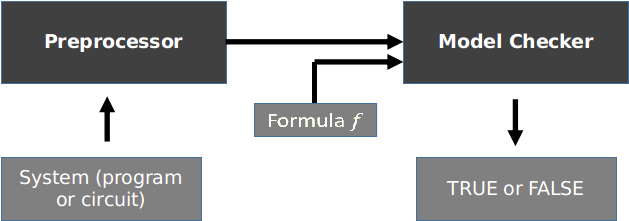
\includegraphics[width=0.8\textwidth]{modelcheckstruc}
\centering
\caption{Model Checker structure (Source: \cite{Clarke2008})}
\label{fig:modelcheckstruc}
\end{figure}

Here it is worth to mention that the term "model" is not the meaning taken from the dictionary. The problem is not dealing with an abstraction of the actual system under study. 

The Fig. \ref{fig:systemverif} shows the process to convert a real system to a model in order to be verified by a model checking. 

\begin{figure}[h]
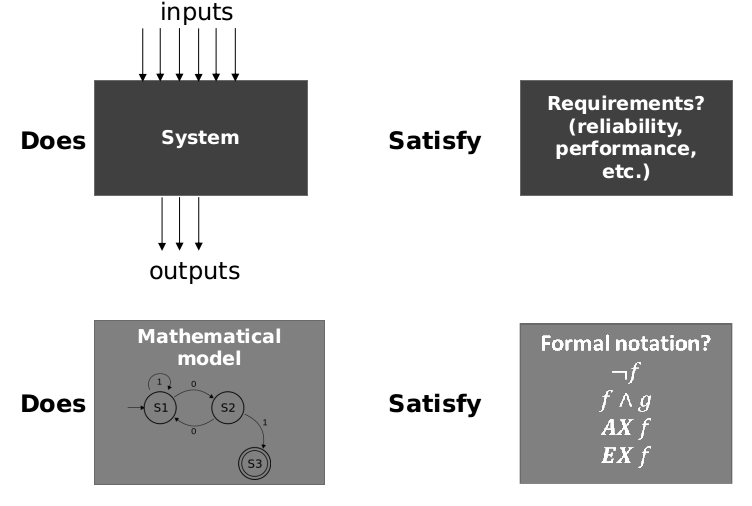
\includegraphics[width=0.8\textwidth]{systemverif}
\centering
\caption{From real system verification to model checking (adapted from \cite{Clarke2008})}
\label{fig:systemverif}
\end{figure}

In order to solve the problem of state explosion, many different techniques were developed at the last decades. One of the promising is the Bounded Model Checking (BMC). 

BMC is a method that checks the model up to a given path in the path length. BMC algorithms traverses a finite state machine for a fixed number of steps, , and checks whether violation occurs with this bound. It uses fast SAT solvers, where SAT means satisfiability. SAT problem, as defined by \cite{Clarke2008}, is a problem of determining if there are certain conditions or interpretation that satisfy a given Boolean expression. SAT solvers are used in BMC, such that if there are some Boolean function, the solver would search the model for conditions (value of variables) that would make the formula $TRUE$. If SAT Solver find a substitution for the formula/function then the substitute induces a counterexample.  

CBMC is considering the best-known model verification tool to validate code in ANSI-C and C++, as can be seen in \cite{Kroening}. 

ESBMC is a context-bounded model checker for embedded C/C++ software based on Satisfiability Modulo Theories (SMT) solver, which can use CBMC as front-end.  
The use of SMT, instead of Boolean Satisfiability SAT from the original BMC, comes as an alternative to overcome limitations of the systems modeling, especially considering that the complexity of these is increasing and the SMT method has high level and richer theories than the SAT to represent the models. 

\subsubsection{ESBMC }
According \cite{GadelhaSBMF}, ESBMC is an open source, permissively licensed (Apache 2), cross platform bounded model checking for C and C++ programs. the efficient SMT based model checker, is a software verification tool for C and C++ code bases. Fig. \ref{fig:esbmcarch} shows the tool architecture. 

\begin{figure}[h]
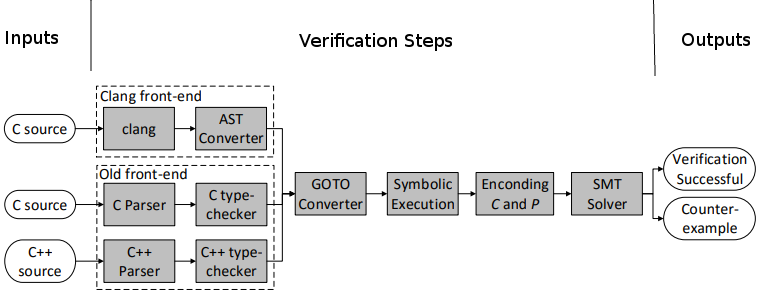
\includegraphics[width=0.9\textwidth]{ESBMCarch2}
\centering
\caption{ESBMC architecture (adapted from \cite{GadelhaSBMF})}
\label{fig:esbmcarch}
\end{figure}

As shown by \cite{GadelhaSBMF}, ESBMC has two alternative front-ends to parse the input program and generate an Abstract Syntax Tree (AST). One legacy CBMC-based front-end that supports both C and C++ and a new clang-based front-end that currently only supports C. The data types and bit vectors are created in the front-end when parsing the code. 

Regardless of the chosen front-end, the output is an AST (tree representation of the abstract syntactic structure of source code written in a programming language) that will be used by the GOTO converter to generate a GOTO program, which has simplified control flow and is suitable for bounded unwinding. The next step is the symbolic execution, when the GOTO program is executed (unrolling loops up to the bound $ k $) and converted to Static Single Assignments (SSA) form. SSA form enables the simplification of algorithms and reduction of computational complexity, where each variable is a target of exactly one assignment statement in the program text. 

During the symbolic execution, ESBMC aggressively tries to simplify the program \cite{Ramalho}; it propagates all constants and solves any assertions that can be statically determined. This is an important step for the verification, since ESBMC can fully verify programs without calling a solver, if the inputs are deterministic. That characteristic is useful at this work to perform the sizing check of the PV system project. 

Following, the SSA expressions are then encoded using the chosen SMT solver supported by ESBMC: Boolector (default) \cite{Brummayer}, Z3 \cite{DeMoura}, MathSAT \cite{Cimatti}, Yices \cite{Dutertre} and CVC4 \cite{Barrett}. 

Finally, the system attempting to determine whether a formula, which is the disjunction of all possible errors, can be satisfied. If the SMT formula is shown to be satisfiable, a counterexample is presented; if the formula is found to be unsatisfiable, there are no errors up to the unwinding bound , and this result is presented. 
 
ESBMC can be invoked through the command-line interface or configured through the Eclipse plug-in. Specific problems and the solver can be selected that way. 

ESBMC aims to support all of ISO/IEC 9899:1999 C programming language standard, and detects errors in software by simulating a finite prefix of the program execution with all possible inputs. Classes of problems that can be detected include: user specified assertion failures, out of bounds array access, illegal pointer dereferences, double-free of malloc'd memory, misaligned memory access; integer overflows, divide by zero, memory leaks, concurrent software, deadlock, and data races (i.e. competing writes). 
 
\subsubsection{Cyber-physical systems x Energy x ESBMC}
According \cite{UC}, cyber-physical systems (CPS) are integrations of computation, networking, and physical processes. Embedded computers and networks monitor and control the physical processes, with feedback loops where physical processes affect computations and vice-versa. The economic and societal potential of such systems is vastly greater than what has been realized, and major investments are being made worldwide to develop the technology. The technology builds on the discipline of embedded systems (computers and software embedded in devices) whose principle mission is not computation, such as cars, toys, medical devices, and scientific instruments. CPS integrates the dynamics of the physical processes with those of the software and networking, providing abstractions and modeling, design, and analysis techniques for the integrated whole. 

Energy production, distribution, and optimization are all CPS problems, mas mentioned in \cite{UC}. For example, the smart grid combines multiple electric power production plants with a multiplicity of loads using dynamic load balancing and dynamic pricing with demand-response strategies. Smart buildings integrate sensors into control systems for lighting, HVAC (heating, ventilation, and air conditioning), and safety (as fire monitoring and evacuation). 

Therefore, in the context of this proposal, a cyber-physical system, specifically a solar photovoltaic system, will be mathematically modeled. Then a model checking will be performed to do a verification of the project in order to guarantee that the design of an off-grid SPV solution will meet the requirements, specifications and regulations. 

As described in \cite{Alur}, in program verification, it is aimed to check if a program satisfies its logical specification. Contemporary verification tools vary widely in terms of source languages, verification methodology, and the degree of automation, but they all rely on repeatedly invoking an SMT solver. This work tracks the same path. 


\section{Methodology }

Fig. \ref{fig:statetransition} shows the state diagram for the proposed framework. 

\begin{figure}[h]
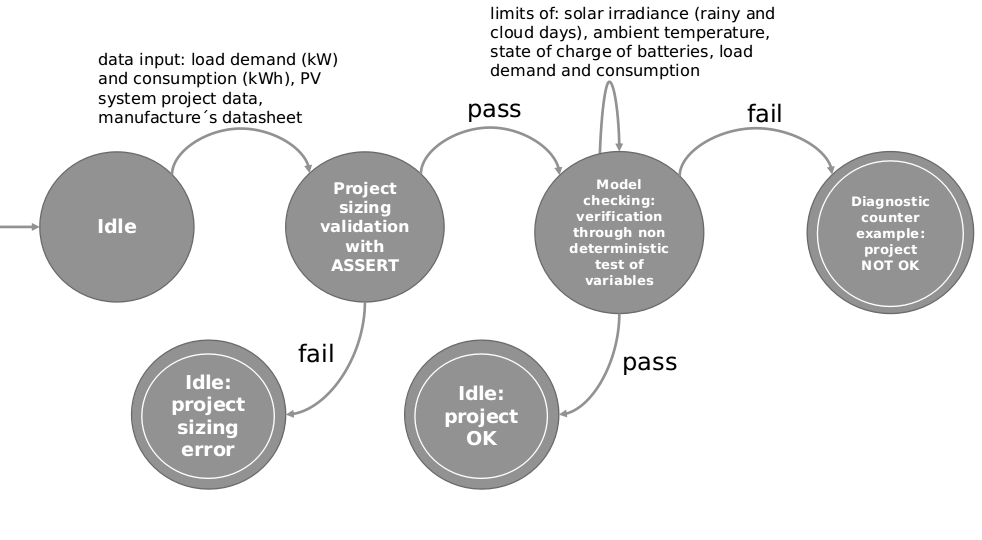
\includegraphics[width=0.8\textwidth]{statetransition}
\centering
\caption{State transition diagram to the proposed framework}
\label{fig:statetransition}
\end{figure}

It is worth mentioning that the steps described here are carried out shortly after the design of the solar photovoltaic system, as soon as the equipment and equipment specifications are defined; before buying and deploying them, as a way to ensure that the project will not fail. 

The PV input data (load power demand, load consumption of energy, the PV system project data, and the manufacturer's data-sheet information), the formulas to check the sizing project, the mathematical model, the limits of the non-deterministic variables of the model, are all written as C Programming language code. 

Then the tool ESBMC is called to perform the verification of this code. The nondeterministic variables (solar irradiance, ambient temperature, state of charge of the batteries, load demand of power and the load consumption of energy) will suffer a heavy test at ESBMC runtime execution. In addition, depending if one of the requirements of the system, as autonomy of the batteries, or the offer of the energy, or even the power supply from the system, is not accomplished or satisfied, the tool accuses a fail, and the diagnostic counterexample shows in which condition the fail/violation happened. 

Simply put, instead of the ESBMC find the defect of a software or if a hardware does not meet the some requirements (as reliability, performance, or safety), the tool will verify if the requirements of the solar PV project are met. Detailing the condition of violation, of not meeting the requirements, if this occurs. 

With this information in hand, the user or the engineer can correct his/her PV project, and run the ESBMC again to insure that the new configuration of the project will work as expected. 

Theorem: XXX  


\section{Results}






\section{Conclusions and Future Work}
The proposed framework seems to be a coherent and promising tool to perform verification of a PV project. The next step is the deployment of the solution at the ESBMC environment, and compare the results with a real PV project deployed at the field. 

The framework presented here establishes the automated verification and the project sizing check. However, it is possible to perform the optimum sizing of the PV system. Moreover, the authors target the use of synthesis to perform the optimum sizing. That is an interesting issue, considering that nowadays is possible to choose from many different manufacturers and many different models of equipment of a SPV system,  the idea of just to validate one given solutions is not enough. Probably is more useful to design a tool which starts from a list of commercial equipments, i.e., inputs, where each equipment is verified during synthesis phase and the final solution, which satisfies the specifications (or constraints) of the project, is found from the inputs, automatically. This is what a Counterexample Guided-Inductive Synthesis (CEGIS) does. 

In the future, it is possible to expand the type of renewable used for power generation. Allowing the verification of wind generation or even hybrid systems, which can transform the tool into an important instrument to complement the solar PV system design process, ensuring that it does not fail and meets the expected requirements. 

Plus (need to think about it): verification in every-hour of a 48h cycle?, PV model math model can be improved, charge/discharge of batteries can be improved (is a simplified model), house's power consumption is not flat or constant, the dweller can buy more home appliances, synthesis need a data base of components, to test peak (surge) consumption (above the nominal), additional models for on-grid/off-grid farm, hybrid, and on-grid with batteries).

%\section{Nomenclature }

text here

%\section{References}

\bibliography{trindadeThesis}{}
%\bibliographystyle{ieeetr}
%\bibliographystyle{model5-names}\biboptions{authoryear}
%\usepackage{numcompress}\bibliographystyle{model4-names}\biboptions{authoryear}
%\printbibliography

\end{document}
